%%%%%%%%%%%%%%%%%%%%%%%%%%%%%%%%%%%%%%%%%
% University/School Laboratory Report
% LaTeX Template
% Version 3.1 (25/3/14)
%
% This template has been downloaded from:
% http://www.LaTeXTemplates.com
%
% Original author:
% Linux and Unix Users Group at Virginia Tech Wiki 
% (https://vtluug.org/wiki/Example_LaTeX_chem_lab_report)
%
% License:
% CC BY-NC-SA 3.0 (http://creativecommons.org/licenses/by-nc-sa/3.0/)
%
%%%%%%%%%%%%%%%%%%%%%%%%%%%%%%%%%%%%%%%%%

%----------------------------------------------------------------------------------------
%	PACKAGES AND DOCUMENT CONFIGURATIONS
%----------------------------------------------------------------------------------------

\documentclass{article}

%\usepackage[version=3]{mhchem} % Package for chemical equation typesetting
\usepackage{siunitx} % Provides the \SI{}{} and \si{} command for typesetting SI units
\usepackage{graphicx} % Required for the inclusion of images
\usepackage{natbib} % Required to change bibliography style to APA
\usepackage{amsmath} % Required for some math elements 
\usepackage[utf8]{inputenc} % Required for special characters processing
%
\usepackage{fullpage} % changes the margin
\setlength\parindent{0pt} % Removes all indentation from paragraphs

\renewcommand{\labelenumi}{\alph{enumi}.} % Make numbering in the enumerate environment by letter rather than number (e.g. section 6)

\usepackage{times} % Uncomment to use the Times New Roman font

%----------------------------------------------------------------------------------------
%	DOCUMENT INFORMATION
%----------------------------------------------------------------------------------------

\title{\textbf{Determination of the Air Adiabatic Constant} \\ Meteorology
  \& Climatology} % Title

\author{Environmental Science Degree} % Author name

\date{\today} % Date for the report

\begin{document}

\maketitle % Insert the title, author and date

\begin{center}
\begin{tabular}{l r}
Date Performed: & \underline{\hspace{3cm}}  \\ % Date the experiment was performed
Partners: & \underline{\hspace{6cm}} \\ % Partner names
& \underline{\hspace{6cm}} \\
& \underline{\hspace{6cm}} \\
Instructor: & Prof.~F.~Pérez-Bernal % Instructor/supervisor
\end{tabular}
\end{center}

% If you wish to include an abstract, uncomment the lines below
\begin{abstract}
In this lab session the R\"uchhardt method is used to measure the
adiabatic coefficient, $\gamma$, of the air.
\end{abstract}

%----------------------------------------------------------------------------------------
%	SECTION 1
%----------------------------------------------------------------------------------------
\section{Introduction}
Due to the low thermal conductivity of the air and the typical time of
most meteorological processes, the buoyant convection and, in general,
most vertical air parcels displacements can be considered as adiabatic
processes. To do so, the following aaproximations are assumed:
\begin{itemize}
\item  The air parcel does not mix appreciably with its surroundings.
\item  Mechanical equilibrium: the parcel pressure adjusts instaneously to pressure changes in the surrounding atmosphere.
\item The parcel temperature does NOT adjust to temperature changes in
  the environment.
\item Energy changes in the macroscopic motion of the parcel are small compared to total energy.
\end{itemize}

An adiabatic process is characterized by the lack of heat
transfer. All temperature changes are associated with exchanges
between internal energy and work, typically through expansion (gas temperature
diminishes) or
contraction (gas temperature increses) of the system. For ideal gases they are modeled by the Poisson equations 
\begin{align}
p \; V^\gamma  &=  \text{Constant,}\\
T \; V^{\gamma-1}  &=  \text{Constant,}\\
T \; p^{-\kappa}  &=  \text{Constant,}
\end{align}
\noindent where $\kappa = 1-\frac{1}{\gamma}$ and $\gamma$ is the
adiabatic coefficient of the ideal gas and it is equal to the ratio of
the molar heat capacity for constant pressure and constant volume,
$\gamma = \frac{C_p}{C_v}$. For diatomic ideal gases $\gamma = 7/5 =
1.4$ and $\kappa = 0.286$.

\section{Objectives}

The objective of this lab session is to \textit{determine the adiabatic
coefficient of the air $\gamma$} using the R\"uchhardt method. This method is
based on the displacement from equilibrium of a piston of mass m that
is released to oscillate in damped simple harmonic motion (see figure \ref{fig_rucchardt}). The
frequency of oscillation is measured and this measurement is combined
with the known physical parameters of the system to estimate
$\gamma$. \textit{The piston is a fragile piece of equipment that
  should be handled with care}. 

\begin{figure}[h]
\begin{center}
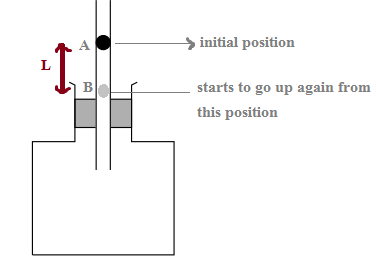
\includegraphics[width=0.5\textwidth]{Figs/upload_2015-6-4_10-54-49.png} % Include the image placeholder.png
\caption{Scheme of the R\"uchhardt method.}\label{fig_rucchardt}
\end{center}
\end{figure}


As a bonus, a second objective of the lab session is to appropriately identify the
\textit{possible sources of errors and your result uncertainty}. 


\section{Theoretical Basis and Lab Procedures}
The harmonic motion of the piston is modeled by the following equation
\begin{equation}
\frac{d^2 z}{d t^2} =  - \, \frac{\pi^2 R^4 p \, \gamma}{m  V} \;
\Delta z~,
\label{harmonic}
\end{equation}
\noindent where $R$ and $m$ are the piston radius and mass, $p$ is the
pressure on the vessel and $V$ is the vessel volume.

From Eq.~\eqref{harmonic} we know that the period of the harmonic
motion, $T$ is
\begin{equation}
T = \frac{1}{2 R^2} \sqrt{\frac{m \; V}{p \; \gamma}}~,
\end{equation}
\noindent and thus, once we measure the period of the vibrations we
can compute $\gamma$ as
{\large
\begin{equation}
\gamma \; = \; \frac{4 \; m \; V}{T^2 \; R^4 \; p}
\end{equation}
}

%----------------------------------------------------------------------------------------
%	SECTION 2
%----------------------------------------------------------------------------------------

\section{Experimental Data}


\textbf{Piston mass:}

\vspace{5mm}

$m\pm E_m = $ \underline{\hspace{4cm}}

\vspace{5mm}


\textbf{Piston diameter and radius:}

\vspace{5mm}

\begin{tabular}{|c|c|c|c|c|}
\hline
$D_1$&$D_2$&$D_3$&$D_4$&$D_5$\\
\hline
~\hspace{3cm}~&~\hspace{3cm}~&~\hspace{3cm}~&\hspace{3cm}~&~\hspace{3cm}~\\
\hline
$R_1$&$R_2$&$R_3$&$R_4$&$R_5$\\
\hline
\hspace{3cm}~&~\hspace{3cm}~&~\hspace{3cm}~&~\hspace{3cm}~&~\hspace{3cm}~\\
\hline
\end{tabular}

\vspace{4mm}

$\overline{R}=\underline{\hspace{4cm}}$
\hspace{1cm}
$\sigma_{\overline{R}}=
\sqrt{\sum_i(R_i-\overline{R})^2\over N(N-1)}=\underline{\hspace{4cm}}$  
\vspace{4mm}

$R\pm E_R = \underline{\hspace{4cm}}$

\vspace{6mm}

\bf{Period of the harmonic motion:}

\vspace{5mm}

Time for 500 oscillations:

\vspace{2mm}

\begin{tabular}{|c|c|c|c|c|}
\hline
$t_1$&$t_2$&$t_3$&$t_4$&$t_5$\\
\hline
~\hspace{3cm}~&~\hspace{3cm}~&~\hspace{3cm}~&\hspace{3cm}~&~\hspace{3cm}~\\
\hline
$T_1=t_1/500$&$T_2$&$T_3$&$T_4$&$T_5$\\
\hline
~\hspace{3cm}~&~\hspace{3cm}~&~\hspace{3cm}~&\hspace{3cm}~&~\hspace{3cm}~\\
\hline
\end{tabular}

\vspace{4mm}

$\overline{T}$ = $\overline{t}$/500 = \underline{\hspace{4cm}}
\hspace{1cm}
$\sigma_{\overline{T}}=\underline{\hspace{4cm}}$
\vspace{5mm}

$T\pm E_T \; = $ \underline{\hspace{4cm}}
\vspace{5mm}


\textbf{Pressure in the vessel:}

\vspace{5mm}

$p_{atm}$ = \underline{\hspace{4cm}} \hspace{1cm} $\frac{m
\; g}{\pi \; \overline{R}^2}$ = \underline{\hspace{4cm}}

\vspace{5mm}

$p \; = \; p_{atm} \; + \; \frac{m \; g}{\pi \;
\overline{R}^2}$ = \underline{\hspace{4cm}}

\vspace{5mm}

$p\pm E_p \; = $ \underline{\hspace{4cm}}

\vspace{5mm}


\textbf{Vessel volume:}

\vspace{5mm}

$V \pm E_V = $ \underline{\hspace{3cm}}
%
%----------------------------------------------------------------------------------------
%	SECTION 3
%----------------------------------------------------------------------------------------


\section{Results and Conclusions}

\vspace{10mm}

\textbf{Air adiabatic coefficient:}

\vspace{5mm}
{\LARGE
$\gamma$ = \underline{\hspace{4cm}}
\hspace{1cm}
$\sigma_{\overline{\gamma}}=\underline{\hspace{4cm}}$
}

\nocite{Smith:2012qr}

%----------------------------------------------------------------------------------------

\bibliographystyle{apalike}

\bibliography{sample}

%----------------------------------------------------------------------------------------


\end{document}
